\section{Problem Model}\label{sec_extrafunc}
The software allocation problem is a type of job shop scheduling with constraints, as such it is a discrete optimization problem \cite{}. The solution to the allocation problem is represented by a vectormatrix $\x=\{\xsp{k}:k=1,...,N_a\}$, where \ttxsp{k} is a matrix of size $N_c\times K$, and \ttssx{x}{k}{ij}$=k\in \{1,…,N_m\}$ represents the mapping of the software component replica \ttssx{c}{k}{ij} to the computation node $m_k$.
\begin{equation}
\label{fig_pso_solution_representation}
\bspx{k}=
\begin{bmatrix} 
\ssx{k}{11} & \ssx{k}{12} & \dots & \ssx{k}{1K}\\
\ssx{k}{21} & \ssx{k}{22} & \dots & \ssx{k}{2K}\\
\vdots & \vdots & \ddots & \vdots\\
\ssx{k}{N_c1} & \ssx{k}{N_c2} & \cdots & \ssx{k}{N_cK}
\end{bmatrix}
\end{equation}

In this work, the main objective of the allocation problem is to satisfy the user-defined requirements, namely reliability requirements, end-to-end timing requirements, and criticality of the software applications $A_i$ by effectively mapping the software components to the computation nodes, $C^{(k)}\mapsto M$. Furthermore, the components are allocated efficiently to minimize the total power consumption $Power(\textbf{x})=\sum_{m\in M'}{P_{m}(\textbf{x})}$ of the applications by selecting lower-power consuming nodes $M'\subseteq M$, provided the requirements are met, where $P_{m}(\textbf{x})$ is the power consumption of node $m$ on the mapping $\textbf{x}$. Power consumption, in this context, refers to the energy usage of electronic components in the integrated circuits of the node, e.g., processor, memory, I/O devices, etc., per time unit. 

%Power consumption refers to the energy usage of electronic components in an integrated circuit, e.g., processor, memory, I/O devices, etc., per time unit. 
There are several power consumption models and different techniques to estimate the power consumption of a computing node. In this work, we employ a technique based on processor load (or \textit{Processor Utilization}) to estimate the average power consumption of a computation node. Specifically, we use the linear polynomial model proposed by Fan et al. \cite{Fan2007PowerComputer}, which is shown in (\ref{eqn_powerconsumption}). The model states that the power consumption of a node is directly proportional to its load, and is inductively formulated from experimental results:
\begin{equation}
\label{eqn_powerconsumption}
f_p(u)=P_{idle} + (P_{busy}-P_{idle})*u,
\end{equation}

where $u$ is the utilization (or load) of a computation node, $p_{idle}$ and $p_{busy}$, respectively, refer to the power consumption of a node measured at minimum and maximum processor loads. Such measurements can be obtained by running performance benchmark suits, e.g., MiBench \cite{Guthaus2001MiBench:Suite}, AutoBench \cite{EMBC2018AutoBenchProcessors}, etc., which is computed based on the utilization of the node via the linear power consumption model shown in Equation (\ref{eqn_powerconsumption}).

Consequently, the power consumption of a node $m$ for a given mapping $\textbf{x}$ is computed using Equations (\ref{eqn_powerconsumption_x}-\ref{eqn_util_component}), by calculating first the node's utilization $U_m(\textbf{x})$ using Equation (\ref{eqn_util_x}). The node's utilization is computed from the set of components allocated to it (which are $\forall_{ij} x_{ij}=m$) using Equation (\ref{eqn_util_x}). And the utilization of a component on the node $m$ is computed from its constituent tasks $T_c$ using Equation (\ref{eqn_util_component}).
\begin{align}
	\label{eqn_powerconsumption_x}
nodPow(\textbf{x}) & =f_p(nodUti(\textbf{x},m))                         &  \\
	\label{eqn_util_x}
nodUtil(\textbf{x},m)           & = \sum_{k}{\sum_{i}{\sum_{j}{comUtil(m,c)}}}|\xkij=m         & \text{, where } c=\sss{C}\\
	\label{eqn_util_component}
comUtil(m,c)              & = \sum_{r\in c.R} \frac{r.e_m}{r.\tau.P}, &
\end{align}

where $c.R$ is set of runnables in component $c$, $r.e_m$ and $r.\tau.P$ are the execution of runnable $r$ on node $m$ and its period, respectively.

The applications requirements are modeled as constraints that need to be satisfied in the allocation problem. The constraints formulations are shown in the following subsections, respectively for reliability, timing and other design constraints such as related to runnables-to-tasks merging and replication.

\subsection{Software Application Reliability Constraints}\label{subsec_reliability_constraint}
The applications reliability constraints ensure the mapping $\textbf{x}$ satisfies the user-defined reliability requirements, that is $ \forall k\in [1,n_A]\ \rel_{A_k}(\xsp{k})\leq RelReq_{A_k}$. 
The reliability  is computed from the execution framework that is provided to run the application, which consists of computation nodes \ttssp{M} and the shared CAN bus B, as shown in Equation (\ref{eqn_appreliability_app}). The nodes \ttssp{M} host the components \ttssp{C} and are determined by searching the mapping \ttxsp{k}  in polynomial time using Equation (\ref{eqn_nodes_app}).
\begin{align}
	\label{eqn_appreliability_app}
	&Reliability_{A_i}(\x)=Reliability_{A_i}(\ssp{M})*Reliability(B)\\
	\label{eqn_nodes_app}
	&\ssp{M}=\{e|e\in M \land \forall ij (e=m_h) \},\mbox{ where } h=\ssx{k}{ij} 
\end{align}

The reliability of the nodes, $Reliability_{A_i}(\ssp{M})$ with respect to the application ${A_k}$ is calculated using the \textit{state-enumeration} technique \cite{Lucet1999ExactReliability}  as shown in Equations (\ref{eqn_appreliability}). According to the technique, the reliability is basically the total probability that the application $A_k$ \textit{functions} under mutually exclusive and uniformly distributed failure-events of the nodes, represented by $\ssp{\mathcal{F}}(\ssp{M})=\{\textbf{0},\textbf{1}\}^{\ssp{M}}$, where  \textbf{0} means node fails, \textbf{1} means  node is operational. An event $\omega\in \mathcal{F}_{A_k}(\ssp{M})$ represents the states of nodes by a sequence of 0-1 variables $(b_1,...,b_n)$, where $\omega.b_i$ denote the state of node $m_i\in \ssp{M}$. %as the state of the nodes $\ssp{M}=\{e_1,...,e_n\}$ by $s\in \ssp{\mathcal{F}}(\ssp{M})=(b_{e_1},...,b_{e_n})$, where $n=|\ssp{M}|$, whereas the state of a node is referenced by $s.b_{e}$.
\begin{align}
\label{eqn_appreliability}
Reliability_{A_i}(\ssp{M})&=\sum_{s\in \ssp{\mathcal{F}}|g(A_i, s)=1}probability(s)
\end{align}

The fact that an application functions $g(A_k, s)$ is defined via its inverse, which is \textit{software application failure}, deductively as follows:
\begin{definition}[Software Application Failure]
The application $A_k$ fails in the event $\omega \in \ssp{\mathcal{F}}(\ssp{M})$ if there exists a component type \ttsss{c} where all of its replica \ttsss{Q} \textit{fail}, otherwise, the application functions, as shown in Equation (\ref{eqn_app_failure}).  A component replica $\sss{q}[k][ij]\in \sss{Q}$ fails if the node that host it $m_h$ fails, where $h=\xkij$.  
\begin{align}
\label{eqn_app_failure}
g(a, \omega)&= 
\begin{cases}
\textbf{0} & \mbox{ if } \exists i\forall j\ (m_h\in \sss{M}[k][\omega] )\\
\textbf{1} & \mbox{ otherwise }
\end{cases}\\
\label{eqn_appreliability_node_s}
\sss{M}[A_k][\omega]&=\{e|e\in \ssp{M} \land (\omega.b_e=1) \},
\end{align}
\end{definition}
where \ttsss{M}[k][\omega] denote the nodes that function at the event $\omega$, and can be found by searching the nodes \ttssp{M} with state $\omega.b_e=1$ in constant time , as show in Equation (\ref{eqn_pro}).

The probability that a nodes-failure event $\omega$ occurs is computed as a product of the probabilities of its consitutuent elements $\omega.b$ as shown in Equation (\ref{label}).
\begin{equation}
\label{eqn_pro}
	\prod_{(m,b)\in (M,\omega)}{\lambda_m*(1-b)+(1-\lambda_m)*b}
\end{equation}
where $\lambda_m$ is the failure-rate of node $m$.

\subsection{Timing constraints}
The timing constraints ensure that the applications are schedulable on the execution platform, that is the tasks and cause-effect chains of each application meet their deadlines. The schedulability of each task is checked using the worst-case response-time anlaysis presented in Subsection \ref{subsec_responsetimeanalysis}, and for the cause-effect chains using delay analysis shown in Subsection \ref{subsec_causeeffectchains}. Before we formulate the timing constraints, first we derive the task graph for a mapping \ttx from the runnables graph \ttsss{g}[k][r], that is using Equation (\ref{eqn_generatetasksgraphs}).  Using Equation (\ref{eqn_uprdaterunnables}), we update the runnables with nodes information, to which they are mapped by traversing elements of the mapping \ttx, $\xkij$, in linear-time complexity $O(n)$, where $n=|\x|*N_r$, and $N_r$ is the total number of runnables in the system. Consequently, we traverse the runnables graphs, and apply the merging rules stated in the Subsection \ref{subsec_autosarsystem} to derive the tasks graphs. In the case that only runnables from the same component are mapped to at least on task, the derivation of tasks graphs is indpedent of the mapping \ttx, and thus can be performed before the mapping activity. However, the tasks graphs has to be updated with the nodes information after the mapping \ttx is identified.
\begin{align}
\label{eqn_uprdaterunnables}
&\forall k,ij\ \forall r\in \sss{H}[k][i,j]\ r.node = n_h& \mbox{, where } h=\xkij\\
\label{eqn_generatetasksgraphs}
&\forall k\ \sss{g}[k][r](\x)\xrightarrow{\text{Eqn. (13);Merging Rules}}\sss{g}[k][\tau](\x)
\end{align}

where $\sss{H}[k][i,j]$ is the set if runnables that implement component $\sss{q}[k][i,j]$.

%To calculate the delay, the response time of tasks is a prerequisite, therefore, the latter is calculated first as follows.

\subsection{Tasks Timing constraints}
The tasks timing constraints states that the worst-case response time of each task in the system meets its respective deadlines for a mapping \ttx, that is $\forall k\forall \tau\in V(g_r(\x))$ $ResponseTime(\tau)\leq Deadline(\tau)$, where $V(\sss{g_r(\x)})$ is the nodes in the tasks graphs. To compute the worst-case response time of the tasks, first we partition the tasks per node, that is tasks mapped to the same node grouped, represented by the $\ssb{T}[n_h]$, by traversing the tasks graphs using Equation (\ref{eqn_tasks_nodes}). The complexity of this equation, considering an adjucency matrix tasks graphs representation is linear-time $O(N_a*n^k)$, where $n$ is the sum of the order and size of graph $\sss{g}[k][\tau](\x)$.
\begin{align}
\label{eqn_tasks_nodes}
T_{m_h}&=\{e | e\in V(\sss{g}[k][\tau](\x)) \land e.node == m_h, \}& \mbox{ for all } h=1,...,n_N
\end{align}

Then, we calculate the response time of each task $\tau \in T_{m_h}$ by invoking the response-time analyais formula and construct the tasks timing constraints as shown in Equation (\ref{eqn_tasks_constraints}).
\begin{align}
\label{eqn_tasks_constraints}
\forall \tau\in T_{m_h} \delta(\tau,m_h)&\leq Deadline(\tau)& \mbox{ for all } h=1,...,\n{M}\\
\end{align}

\subsection{Cause-effect Chains Timing constraints}
For a mapping \x, the age delays of cause-effect chains should meet thier respective end-to-end requirements, that is $\forall k\forall ij\ AgeDelay_\Gamma(\x)\leq \sss{E2eReq}[k][\Gamma]$, where $\Gamma\in \sss{\Gamma}$. To calculate the age delays, first we identify the messages scheduled by the CAN bus for the mapping \ttx using Equation (\ref{eqn_messages}). 
\begin{align}
\label{eqn_messages}
	M=\{e|\forall (a,b)\in g_\tau(\x)\forall n\in N\ (a\mapsto n \land b\mapsto n=false)\implies createMsg(e)\},
\end{align}
where $Period(e)=Period(a)$, that is the message inherits the period of its predecessor (or sender) task. Accordingly, we update only the chains that communicate over the shared CAN bus to incorporate the messages, that is $\sss{\Gamma}=\{\sss{\Gamma}[k][1],e^*,\sss{\Gamma}[k][N]\}$, where $e\in V(g_\tau(\x))\cup M$. Using Equation (\ref{eqn_agedelay}), we calculate the age delays of each cause-effect chains. 



\subsection{Software Allocation Optimization Problem	}\label{sec_allocation}
In this section, we define the allocation problem of a fault-tolerant software application on a network of heterogeneous nodes which is formulatd as ann optimization problem as shown in Equation (\ref{eqn_const_func}). The optimization problem considers minimizing of power consumption $p(x)$ as the objective while fulfilling timing (\ref{eqn_timing}) and application reliability requirements (\ref{eqn_reliability}) of the software applications as well as satisfying design and hardware constraints, e.g., respecting affinity of software components to dedicated nodes.
\begin{align}
\label{eqn_optimization}
\min_{x\in X}\;\;& P(\textbf{x}) & \\
\text{Subj to:} &\\
& ResponseTime_i(\textbf{x}) \leq Deadline_i & \text{for }\tau_i\in T, i=1,2,...,N_\tau \\ 
\label{eqn_e2e}
&Delay_i(\textbf{x}) \leq EndToEnd_i & \text{for }\Gamma_i\in \Gamma, i=1,2,...,N_\Gamma \\
\label{eqn_reliability}
&Reliability_i(\textbf{x}) \leq RelReq_i & \text{for }a_i\in A, i=1,2,...,N_A\\
\label{eqn_mapping}
&StaticMapping_i(\textbf{x})\models \top & \text{for }c_i\in C, i=1,2,...,N_c
\end{align}
where $x\in X$ is a feasible solution from the search space
$X$, is the search space of the problem,  are a set of timing specification constraints, $Timing\in \Bbb R^n$ is a set of timing boundaries, and $c^{reliability}\in \Bbb R^n$ is a set of reliability boundaries.

In the rest of this section, we show the ILP model and the PSO algorithm of the software allocation problem, which are validated on an automotive use case and evaluated for performance in the next section. Throughout this section, we use a simple running example of a system model in order to demonstrate our proposed ILP model and the PSO optimization algorithm.

\subsection{Running Example}
The example employs an AUTOSAR system, which consists of a software application model and a hardware platform model, as well as functional and extra-functional requirements such as timing and reliability of the software application. The software application is modeled as a digraph of runnables, which is shown in Figure \ref{fig_application}. It consist of 50 runnables, 35 cause-effect chains (or paths), with their activation patterns and timing specifications shown in Table \ref{tbl_requirements}. The timing specifications of the runnables as well as the software components from which the runnables are instantiated are shown in Table \ref{tbl_comps_config}. The hardware platform model consists of three computation nodes, with specifications shown in Table \ref{tbl_nodes_specification}.
\begin{figure}[t!]
\centering
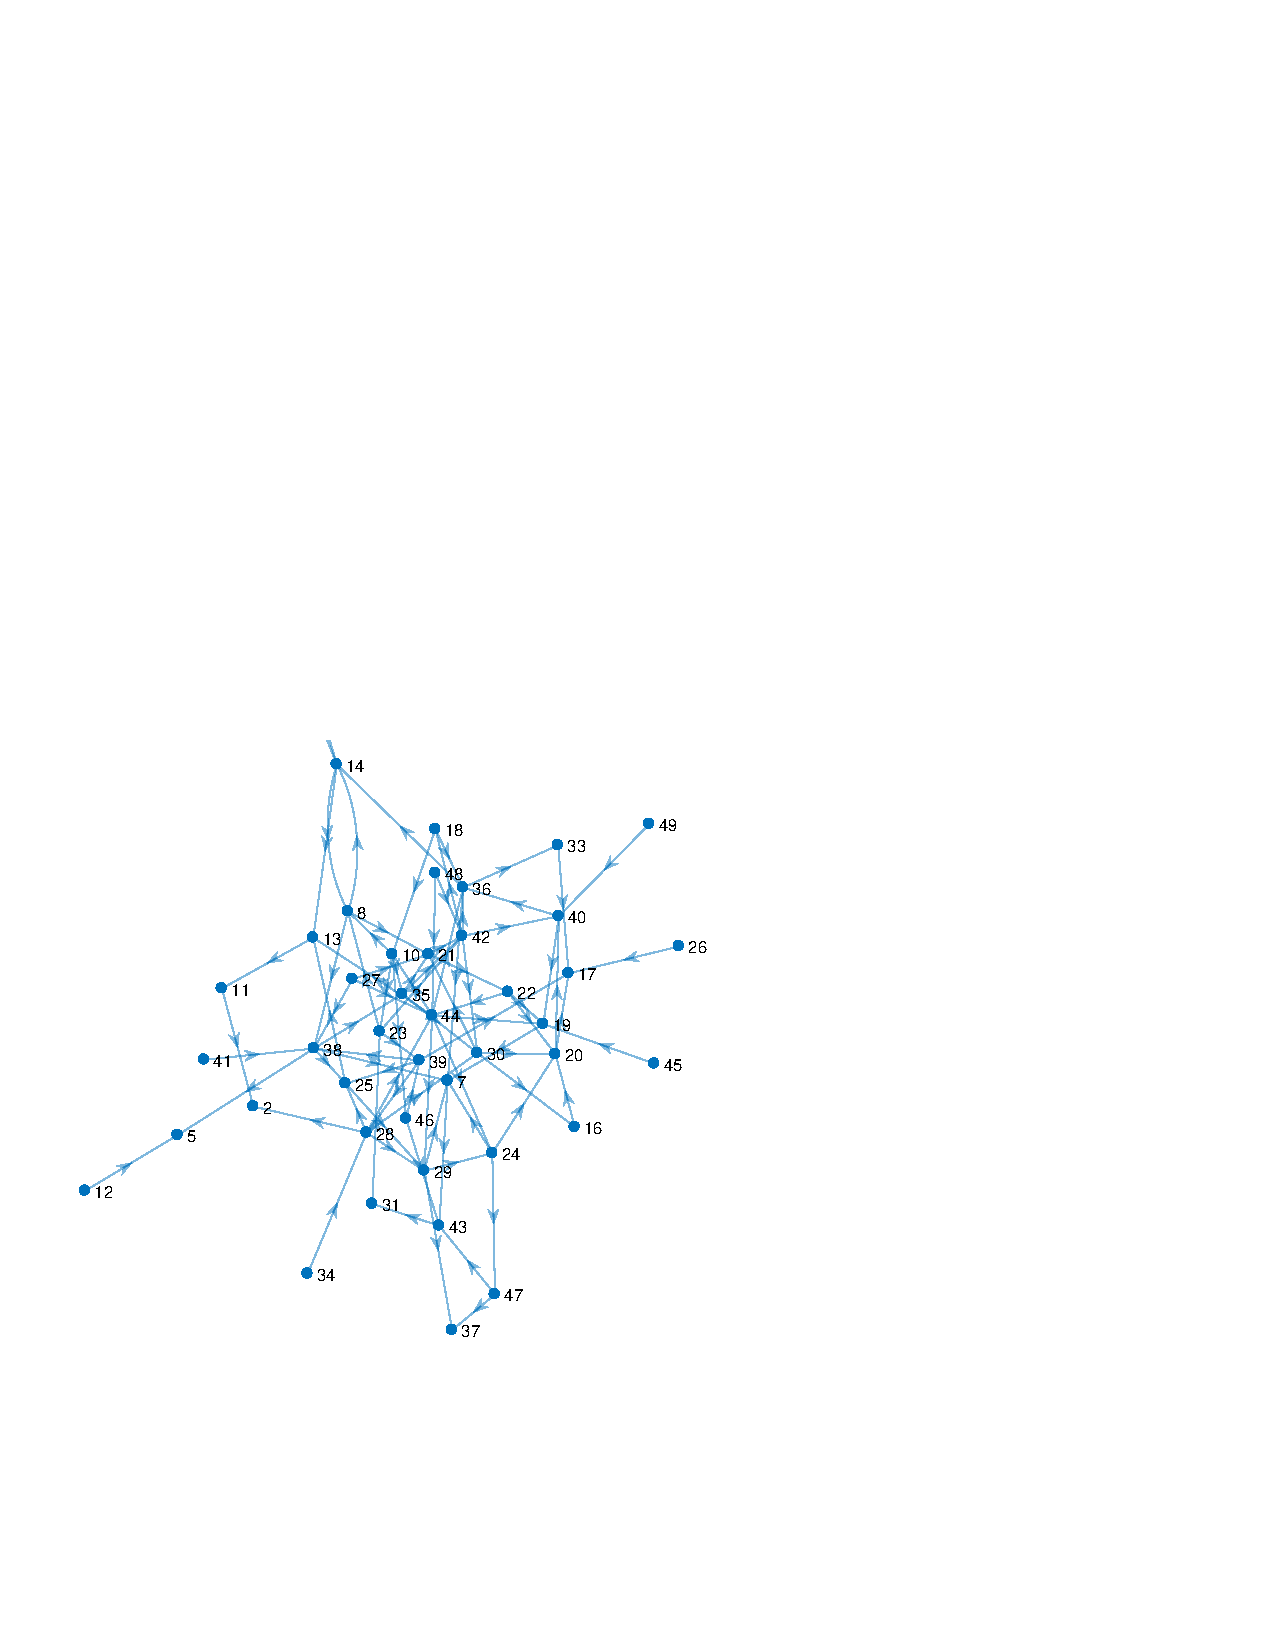
\includegraphics[width=0.8\linewidth]{dag}
\caption{A Directed Acyclic Graph of the Running AUTOSAR Software Application, Runnables = 50, Paths = 35, Activation Patterns shown in Table \ref{tbl_requirements}.}
\label{fig_application}
\end{figure}
\begin{center}
\small
\begin{minipage}{.5\textwidth}%
\centering
\begin{tabular}{@{}p{0.25cm}lll@{}}
\toprule
C& $r_i$ & $(e_{r_im_1}, e_{r_im_2}, e_{r_im_3})$ & $period$\\ \midrule
\multirow{4}{4em}{c1} 
&$r_1$ & (0.030, 0.060, 0.090) & 1\\
&$r_2$ & (0.041, 0.081, 0.122) & 2\\
&$r_3$ & (0.083, 0.167, 0.250)  & 5\\ 
&$r_4$ & (0.310, 0.620, 0.930) & 10 \\[0.3em]
\hline
\multirow{2}{4em}{c2} 
&$r_1$ & (0.310, 0.620, 0.930) & 10\\
&$r_2$ & (0.310, 0.620, 0.930) & 10\\
&$r_3$ & (0.310, 0.620, 0.930)  & 10\\ 
&$r_4$ & (0.310, 0.620, 0.930) & 10 \\[0.3em]
\hline
\multirow{2}{4em}{c3} 
&$r_1$ & (0.310, 0.620, 0.930) & 10\\
&$r_2$ & (0.291, 0.583, 0.874)) & 10\\
&$r_3$ & (0.291, 0.583, 0.874)  & 20\\ 
&$r_4$ & (0.291, 0.583, 0.874) & 20 \\[0.3em]
\hline
\multirow{2}{4em}{c4} 
&$r_1$ & (0.291, 0.583, 0.874) & 20\\
&$r_2$ & (0.291, 0.583, 0.874)) & 10\\
&$r_3$ & (0.291, 0.583, 0.874)  & 20\\ 
&$r_4$ & (0.093, 0.186, 0.279) & 50 \\[0.3em]
\hline
\multirow{2}{4em}{c5} 
&$r_1$ & (0.420, 0.841, 1.261) & 100\\
&$r_2$ & (0.420, 0.841, 1.261)) & 100\\
&$r_3$ & (0.420, 0.841, 1.261)  & 100\\ 
&$r_4$ & (0.420, 0.841, 1.261) & 100 \\[0.3em]
\bottomrule
\end{tabular}
\captionof{table}{Specification of Components.}
\label{tbl_comps_config}
\end{minipage}~
\begin{minipage}{.45\textwidth}
\begin{center}
    \begin{tabular}{@{}lll@{}}
    \toprule
    Activation, $AP$ & Share & Time, ms \\ \midrule
    $\tau_1$ & 50  & 50\\
    $\tau_1\rightarrow\tau_2$ & 20  & 100\\
    $\tau_1\rightarrow\tau_2\rightarrow\tau_3$ & 20  & 200\\
    $\tau_1\rightarrow\tau_2\rightarrow\tau_3\rightarrow\tau_4$ & 10  & 400\\
    \bottomrule
    \end{tabular}
    \captionof{table}{Activation Patters of Cause-effect Chains, their Share and End-to-end Timing Requirements.}
    \label{tbl_requirements}
\end{center}
\begin{center}
    \begin{tabular}{@{}llll@{}}
    \toprule
    M  & $P_{idle}$& $P_{busy}$& $\lambda$ \\ \midrule
    $m_1$ & 50.0& 140.0 &1.0E-3  \\
    $m_2$ & 10.0& 100.0 &1.0E-4  \\
    $m_3$ & 10.0& 140.0 &1 .0E-5 \\ \bottomrule
    \end{tabular}
    \captionof{table}{Computation Nodes Specification.}
    \label{tbl_nodes_specification}
\end{center}
\end{minipage}
\end{center}

In the next subsequent subsections, we propose a metaheuristic approach which is based on Particle Swarm Optimization (PSO) and hybrid PSO. Furthermore, we elaborate the approach using the presented running example.
